\section{Consistency and Rates for Clustering with DBScan}

There is a simple and efficient modification of the DBSCAN algorithm that can detect the most interesting vertical threshold level in an automated way with consistency and optimal learning rates.

The clustering algorithm approximates the optimal level $\rho^*$ and estimates the corresponding clusters by using a kernel density estimator. 

\begin{figure}[H]
    \centering
    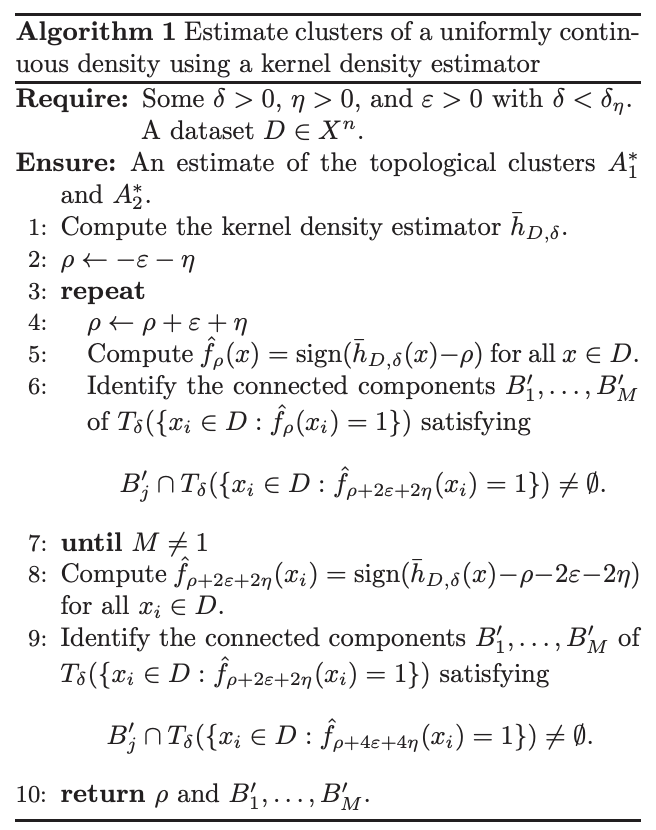
\includegraphics{chapter_2/files/consistency_dbscan.png}
    \caption{The algorithm here loops until it is able to find a level where there is more than one connected component. Then it returns the optimal level and the corresponding clusters.}
    \label{fig:consistency_dbscan}
\end{figure}

\section{Robustness Guarantees for Density Based Clustering}
    
    Very recently, there has been work done to show that a modified version of DBSCAN (Robust DBSCAN) can be shown to have robustness and consistency guarantees against possible (adversarial) contamination. An example to show how applicable this is can be taken from \cite{pmlr-v89-jiang19a}, where there are several horizontal and vertical white lines across an image. Robust DBSCAN can perform the image segmentation while DBSCAN over segments the image due to the corruption.
    
    \begin{figure}[H]
        \centering
        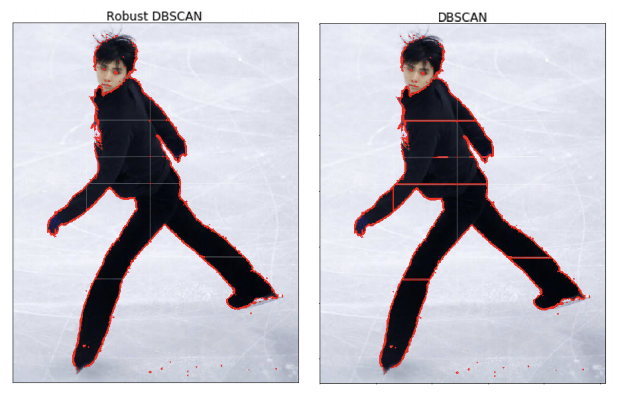
\includegraphics{chapter_2/files/Robustness_Skater_Example.png}
        \caption{The image of the skater corrupted with white lines is over segmented by DBSCAN, but segmented in a more believable way by the Robust DBSCAN.}
        \label{fig:robust_skater}
    \end{figure}
    
    
    Another good example of another case of the strengths of robust DBSCAN is the following classification results against adversarially designed data:
    
    \begin{figure}[H]
        \centering
        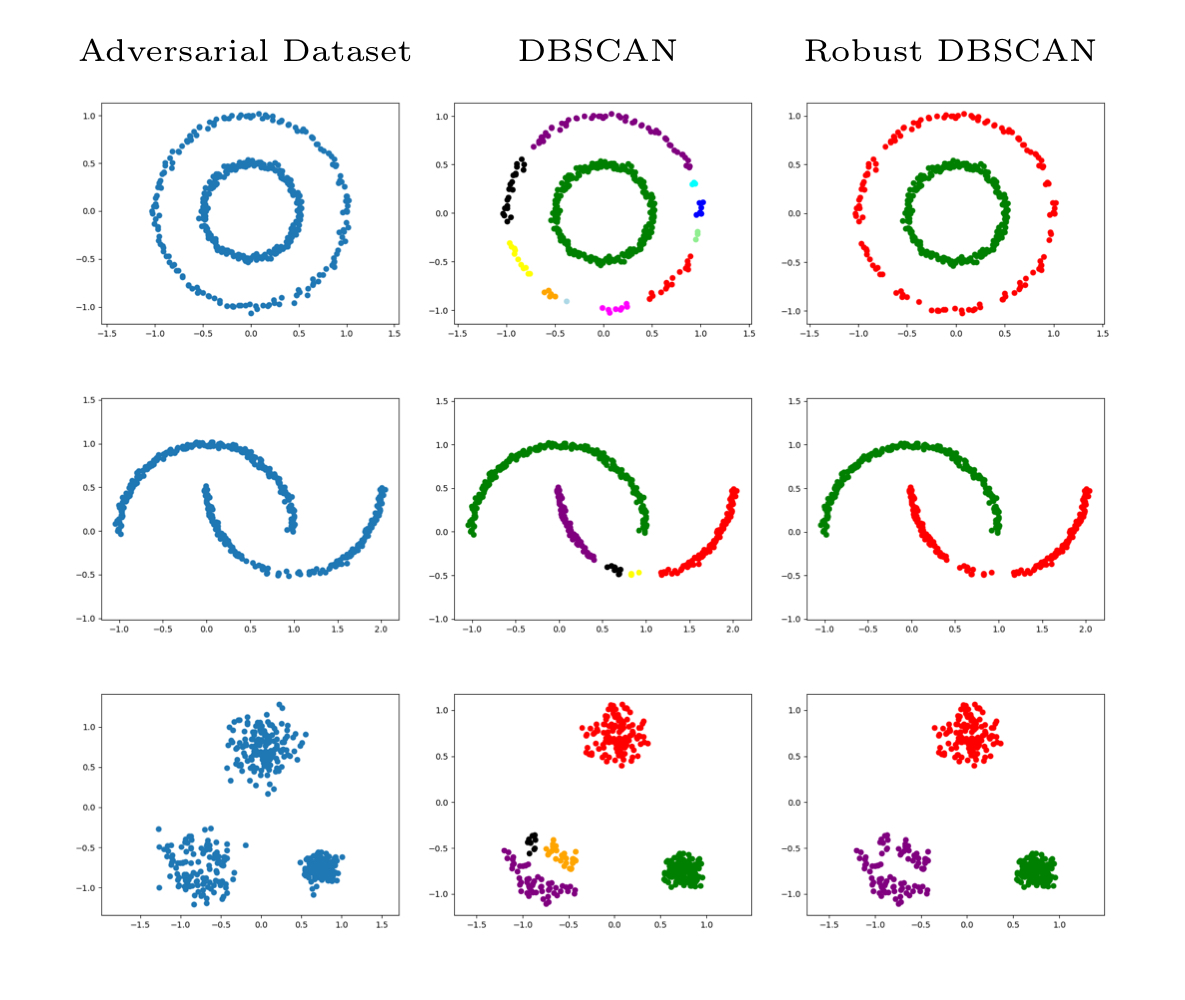
\includegraphics[width=0.9\textwidth]{chapter_2/files/adverse_data.jpeg}
        \caption{We see that the DBSCAN algorithm performs poorly on the adversarially designed data while the Robust DBSCAN algorithm performs better.}
        \label{fig:robust_data}
    \end{figure}
    
  \begin{algorithm}[H]
    \caption{Robust DBSCAN}
    \label{dbscan++ alg}
    \begin{algorithmic}[1]
      \renewcommand\algorithmicrequire{\textbf{Input}}
      \REQUIRE $X = {x_1\cdots x_n}$, $\epsilon, \tilde{\epsilon} \in \bbR^+$, $k \in \mathbb{N}$
      \STATE H := $\{x \in X \ : \ |X \cap B(x, \epsilon)| \geq k\}$
      \STATE D := DBSCAN(X,$\tilde{\epsilon}$,k)
      \STATE C := $\{ C \cap H : C \in D \}$
    \end{algorithmic}
  \end{algorithm}
  
  The main difference with this algorithm is that we are taking an $\tilde{\epsilon}$-neighborhood graph instead of a $\epsilon$-neighborhood graph where we choose $\tilde{\epsilon}>\epsilon$. 
  
  
  As a whole the paper aims to provide certain guarantees:
  \begin{enumerate}
      \item If the hyper-parameters are chosen appropriately depending on the number of samples $n$, and the number of possibly adversarial added samples, $l$ , then with high probability, the number of clusters will not change when adding these samples and that furthermore, there exists a one-to-one correspondence between the clusters and obtained on the original data-set and the clusters obtained on the contaminated data-set such that the distances between the corresponding clusters is bounded. 
      \item Then it is shown that if the data has a E-fraction of contamination (i.e. $l \approx E \cdot n$) with sufficiently small E, then as the number of points that we are considering goes to infinity, the procedure is robust up to an error of $\mathcal{O}(E^{\alpha/(\beta\cdots\alpha+\beta\cdot D)})$  where D is the dimension of the data.
  \end{enumerate}
  
  To derive these results we consider the following assumptions:
  
  \begin{enumerate}
      \item Given regularity assumptions, the density has smoothness (i.e. Holder Continuous) and that the levels sets are smooth w.r.t to the level.
      \item We first establish guarantees on the core points and how they are chosen by the two algorithms to show that are mostly the same
      \item Then we establish guarantees on the clusters that are chosen by the algorithms and show they are largely the same.
  \end{enumerate}

\begin{remark} (Smoothness).
Let $0<\alpha\leq 1$. There exists constant $C_{\alpha}>0$ such that $|f(x)-f(x')|\leq C_{\alpha}\cdot|x-x'|^{\alpha}$
\end{remark}

\begin{remark} (Level-Set).
The $\lambda$-level set of f is defined as $L_f(\lambda) := \{ x \in \mathcal{X}: f(x)\geq \lambda \}$
\end{remark}

\begin{remark} ($\ominus$).
The $\epsilon$-interior of A is defined as $A \ominus \epsilon := \{ x \in A, \inf\limits_{y \in \partial A}d(x,y)\geq \epsilon \}$ where ($\partial$ A is the boundary of A).
\end{remark}

\begin{remark} (Curvature).
There exists $C_\beta > 0$ and $\beta > 0$ such that the following holds. For any $0<\lambda \leq \lambda'<||f||_{\infty}$, we have $L_f(\lambda)\ominus(i(|\lambda'-\lambda|)) \subseteq L_f(\lambda')$
\end{remark}

\begin{fact}
(k-NN Density Estimator). Define the k-NN radius of $x \in \mathbb{R}^D$ as $r_k(x):=\inf\{r>0:|X\cap B(x,r)|\geq k\}$. Then the k-NN density estimator is:
\begin{equation*}
    f_k(x):=\frac{k}{n\cdot v_D \cdot r_k(x)^D}
\end{equation*}

where $v_D$ is the volume of a unit ball in $\mathbb{R}^D$.
\end{fact}

Given the k-NN Density Estimator, we have the following high probability guarantee.

\begin{lemma} (k-NN density estimation rates). Let $0<\delta<1$. Suppose that f satisfies the assumption for smoothness. Then the following holds for some constants C and $C_l$ depending on $f$. Suppose k satisfies

\begin{equation*}
    k\geq C_l\cdot\log(1/\delta)^2\cdot\log(n)
\end{equation*}

Then with probability at least $1-\delta$,

\begin{equation*}
    \sup\limits_{x\in \mathcal{X}}|f(x)-f_k(x)| \leq C \cdot \left(\frac{\log(1/\delta)\sqrt{\log n}}{\sqrt{k}} + \left(\frac{k}{n}\right)^{\alpha/D}\right)
\end{equation*}
\end{lemma}

The first guarantee that can be given is that when running algorithm on X vs running with $l$ additional samples, the new core points will appear near the original core points:

\subsection{Guarantees on Core Points}

\begin{theorem}
Given that our assumptions are met on the smoothness and curvature of $f$ such that the following holds. Let $0<\delta<1$ and $k$ satisfy:

\begin{equation*}
    k\geq C_l\cdot\log(1/\delta)^2\cdot\log(n) + l
\end{equation*}

and $\tilde{\epsilon}\geq\epsilon>0$. Let $\hat{C}$ and $\hat{C'}$ be the core-points returned by the robust DBSCAN algorithm when run on X and X' respectively. With probability at least $1-\delta$,

\begin{equation*}
    \hat{C'}\subseteq \hat{C}\oplus\tilde{r}
\end{equation*}

where $\oplus$ denotes a tube around a set (i.e. $A \oplus r := \{x\in\mathcal{X}: \inf_{a\in A}|x-a|\leq r\}$), and
\begin{equation*}
    \tilde{r}:=C\cdot\left(\left(\frac{l}{n\epsilon^D}\right)^{\frac{1}{\beta}} + \frac{\log(1/\delta)^{\frac{1}{\beta}}\cdot(\log n)^\frac{1}{2\beta}}{(k-l)^{\frac{1}{2\beta}}} + \left(\frac{k}{n}\right)^{\frac{\alpha}{\beta\cdot D}}\right)
\end{equation*}
\end{theorem}\\

\textit{Proof:} The key ideas in this proof is to leverage our lemma and our assumptions in order to bound a quantity that will ensure that there are no new core points created.

This is the proof that we are going to dissect:

First we want to define the outputs from the Robust DBSCAN algorithm given that it received the original X data points and X' (X with $l$ additional samples).

\begin{align*}
\hat{C} &= \{x \in X: |B(x,\epsilon) \cap X|\geq k \}\\
\hat{C'} &= \{x \in X': |B(x,\epsilon) \cap X'|\geq k \}
\end{align*}

Being labeled as a core point is equivalent to $r_k(x) \leq\epsilon$ (where $r_k(x)$ is the k-NN radius of any point). That means those that are not core points must have $r_k(x) > \epsilon$. Therefore if we can show that if:

\begin{equation*}
    \inf\limits_{x\in\mathcal{X} \textbackslash (\hat{C}\oplus\tilde{r})} r_{k-l}(x)>\epsilon
\end{equation*}

Then we can show that $\hat{C'}$ is reliably a subset of $\hat{C}\oplus\tilde{r}$. 

We use $r_{k-l}$ since after inserting l points, we can decrease the k-NN radius of any point up to its $(k-l)$-NN radius (trivially we can achieve this by placing our new points very close to x).

Leveraging our lemma about the k-NN density neighbor estimator while knowing that $r_k(x)\leq \epsilon$ (which directly implies $f_k(x) \geq \frac{k}{nv_D\epsilon^D}$) also implies $x\in\hat{C}$. We can have the following hold for some constant $C_1>0$ depending on $f$. Then for $x \in \hat{C}$ we have:

\begin{equation*}
    f(x) \geq \frac{k}{nv_D\epsilon^D} +  C_1 \frac{\log(1/\delta)\sqrt{\log n}}{\sqrt{k}} + C_1\left(\frac{k}{n}\right)^{\alpha/D}
\end{equation*}

Therefore using our level set notation we can write this idea as:

\begin{equation*}
    L_{f}(A_k) \subseteq \hat{C}
\end{equation*}

Therefore in order to show our original expression, it is equivalent to show that:

\begin{equation*}
    \inf\limits_{x\in\mathcal{X} \textbackslash (L_{f}(A_k)\oplus\tilde{r})} r_{k-l}(x)>\epsilon
\end{equation*}

We can then invoke the curvature assumption in order to rewrite the condition for the level set. We claim that $f(x)\geq A_k-C_{\beta}\cdot\tilde{r}^{\beta}$ implies that $x \in L_{f}(A_k) \oplus \tilde{r}$. Therefore, it is enough to show that:

\begin{equation*}
    \inf\limits_{x\in\mathcal{X} \textbackslash (L_{f}(A_k - C_{\beta}\tilde{r}^{\beta})} r_{k-l}(x)>\epsilon
\end{equation*}

We can re-write this as

\begin{equation*}
    \sup\limits_{x\in\mathcal{X} \textbackslash (L_{f}(A_k - C_{\beta}\tilde{r}^{\beta})} f_{k-l}(x)<\frac{k-l}{n\cdot v_D\cdot \epsilon^D}
\end{equation*}

If we apply that k-NN density estimation bounds from our lemma again, we have for some constant $C_2>0$ depending on f. (Combined with $f(x)\geq A_k - C_{\beta}\cdot\tilde{r}^{\beta}$)
\begin{equation*}
    \sup\limits_{x\in\mathcal{X} \textbackslash (L_{f}(A_k - C_{\beta}\tilde{r}^{\beta})} f_{k-l}(x)\leq A_k - C_{\beta}\tilde{r}^{\beta}+ \frac{C_2\log(1/\delta)\sqrt{\log n}}{\sqrt{k-l}} + C_2\left(\frac{k}{n}\right)^{\alpha/D}
\end{equation*}

In order to have our two conditions agree, we then have:

\begin{equation*}
    C_{\beta}\tilde{r}^{\beta} \geq \frac{l}{n\cdot v_D\cdot \epsilon^D} + \frac{(C_1+C_2)\log(1/\delta)\sqrt{\log(n)}}{\sqrt{k-l}} + (C_1+C_2)\left(\frac{k}{n}\right)^{\alpha/D}
\end{equation*}

which will hold for a sufficiently large choice of C as desired.

\subsection{Guarantees on Clusters}

Our first result bounds the distance between the new core points that appear after adding $l$ samples and the original core points. With this distance guarantee, we can show that the original clustering remains after the addition of $l$ new samples.

\begin{theorem}
Suppose that the conditions of Theorem 1 hold. Let $\mathcal{C}$, $\mathcal{C'}$ be output of the Robust DBSCAN algorithm on $X$ and $X'$ respectively and define the minimum inter-cluster distance of the returned clusters $R:=\min_{C_1,C_2 \in \mathcal{C}} \min_{x_1 \in C_1, \: x_2 \in C_2} d(x_1,x_2)$. If additionally the following holds:

\begin{equation*}
    \tilde{r}\leq \tilde{\epsilon}\leq \frac{1}{2}R-\tilde{r}
\end{equation*}

Then $|\mathcal{C}|=|\mathcal{C'}|$ (i.e. the number of clusters does not change) and there exists a one-to-one mapping of the clusters $\sigma: \mathcal{C} \rightarrow \mathcal{C'}$ such that $C\subseteq \sigma(C)$ for all $C\in \mathcal{C}$ (i.e. original clusters are preserved).
\end{theorem}\\

\textit{Proof:} We know that by the first theorem that all new points in $\mathcal{C}'$ will be at a distance at most $\tilde{r}$ from a point appearing originally in $\mathcal{C}$. Therefore if $\tilde{\epsilon}\geq\tilde{r}$, then these new points will automatically become reconnected to a cluster in $\mathcal{C}$. Also since $\tilde{\epsilon}\leq\frac{1}{2}R-\tilde{r}$, this means that no two distinct clusters in $\mathcal{C}$ will become merged in $\mathcal{C}'$.

These results are then further extended to recover bounds (under the Hausdorff metric) between clusterings of data with the Robust DBSCAN algorithm given a specific proportion of inserted points ($0<E<1$).